\section{Development}

\subsection{Version 1}

\subsubsection{Strategy}

The initial version of the parallel implementation sought to parallelise the main update loop in the serial implementation, shown in Figure \ref{fig:serialloop}. This was achieved by splitting up the elements in the matrix evenly (or as close to evenly as possible) into $p$ batches. This will ensure that (provided threads are never blocked from running) all threads are busy for approximately the same amount of time. Then, it was possible to iterate over these chunks of the problem as in the serial implementation to update the main matrix. This still relies on taking a temporary copy of the main matrix. In order to ensure that no concurrent writes could occur, I used a \texttt{pthread\_mutex\_t} to guard access to the main matrix.

Test runs for Version 1 were completed using multiples of 20 for the value of $p$ in the interval $[20, 160]$.

\begin{figure}[H]
    \centering
    \begin{lstlisting}[language=C]
    for (size_t i = 1; i < size - 1; i++) {
        for (size_t j = 1; j < size - 1; j++) {
            double meanValues[] = {
                copy[i - 1][j],
                copy[i][j + 1],
                copy[i + 1][j],
                copy[i][j - 1]
            };
            mat[i][j] = doubleMean(meanValues, 4);
            if (fabs(mat[i][j] - copy[i][j]) > PRECISION) {
                stop = false;
            }
        }
    }
    \end{lstlisting}
    \caption{Element Update Loop of Serial Implementation}
    \label{fig:serialloop}
\end{figure}

\subsubsection{Analysis} \label{v1results}

The average elapsed time using $p$ threads is shown in Table \ref{tab:timev1}, and measured in terms of Speedup, Efficiency, and Karp-Flatt in Table \ref{tab:metricsv1}. This is visualised in Figures \ref{fig:Sp1}, \ref{fig:Ep1}, and \ref{fig:kf1}. It was evident from the Efficiency and Karp-Flatt scores for this implementation that core utilisation was low. This indicates that there was significant work being executed serially. Investigation into the implementation revealed two bottlenecks.

The first bottleneck was due to the serial nature of the write operation. That is, the main matrix was locked as a whole for the write of an individual element. So, despite the fact that there were (assuming maximal thread use) $p$ values being calculated simultaneously, the locking of the main matrix in memory meant that only one value could be written at once, resulting in $O(N)$ time complexity. Assuming perfectly parallel speedup for the read operation, this would give a complexity $O(\frac{N}{p} + N)$.

The second bottleneck related to the read operation, which was implemented serially in its entirety from the outset. It is likely that the overhead of this was non-trivial, and was dominating the run time. Assuming perfectly parallel speedup for the write operation, this would give an overall complexity $O(N + \frac{N}{p})$.

In addition to the limitations described above, it can be observed that there is a significant dropoff in speedup after a peak using 40 threads. It is likely that this dropoff is caused by the overhead of orchestrating moving data between nodes, as the HPC cluster has a maximum of 44 tasks per node. In cases where more than 44 threads are used, this overhead may have been dominating the run time.

\begin{table}[H]
    \centering
    \begin{tabular}{cc}
    \textbf{Threads ($p$)} & \textbf{Elapsed Time ($t_p$) / s} \\ \hline
    20 & 236.400 \\
    40 & 215.908 \\
    60 & 224.479 \\
    80 & 224.343 \\
    100 & 227.028 \\
    120 & 228.926 \\
    140 & 233.928 \\
    160 & 238.610
    \end{tabular}
    \caption{Mean Elapsed Time using $p$ Threads for Version 1}
    \label{tab:timev1}
\end{table}

\begin{table}[H]
    \centering
    \begin{tabular}{cccc}
    \textbf{Threads ($p$)} & \textbf{Speedup ($S_p$)} & \textbf{Efficiency ($E_p$)} & \textbf{Karp-Flatt Metric ($e$)} \\ \hline
    20 & 2.439 & 0.122 & 0.357 \\
    40 & 2.670 & 0.067 & 0.349 \\
    60 & 2.568 & 0.043 & 0.372 \\
    80 & 2.570 & 0.032 & 0.376 \\
    100 & 2.540 & 0.025 & 0.384 \\
    120 & 2.519 & 0.021 & 0.389 \\
    140 & 2.465 & 0.018 & 0.399 \\
    160 & 2.416 & 0.015 & 0.408
    \end{tabular}
    \caption{Speedup, Efficiency, and Karp-Flatt Metrics using $p$ Threads for Version 1}
    \label{tab:metricsv1}
\end{table}

\begin{figure}[H]
    \centering
    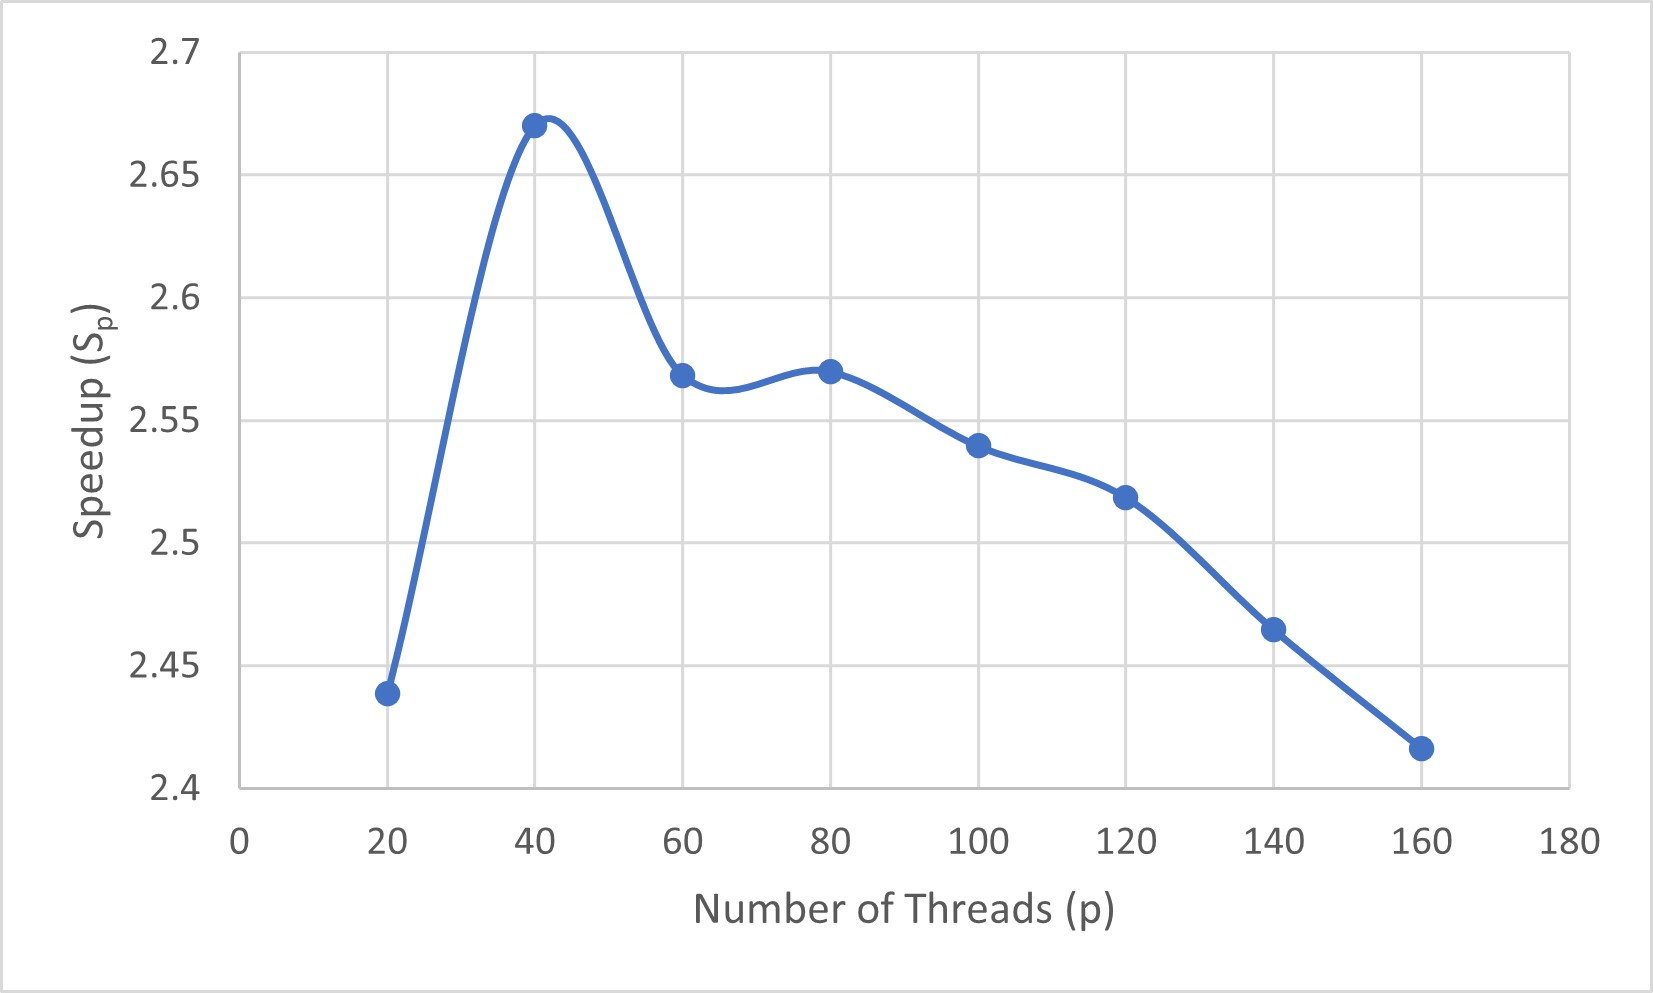
\includegraphics{Sp1}
    \caption{Graph of Speedup using $p$ Threads for Version 1}
    \label{fig:Sp1}
\end{figure}

\begin{figure}[H]
    \centering
    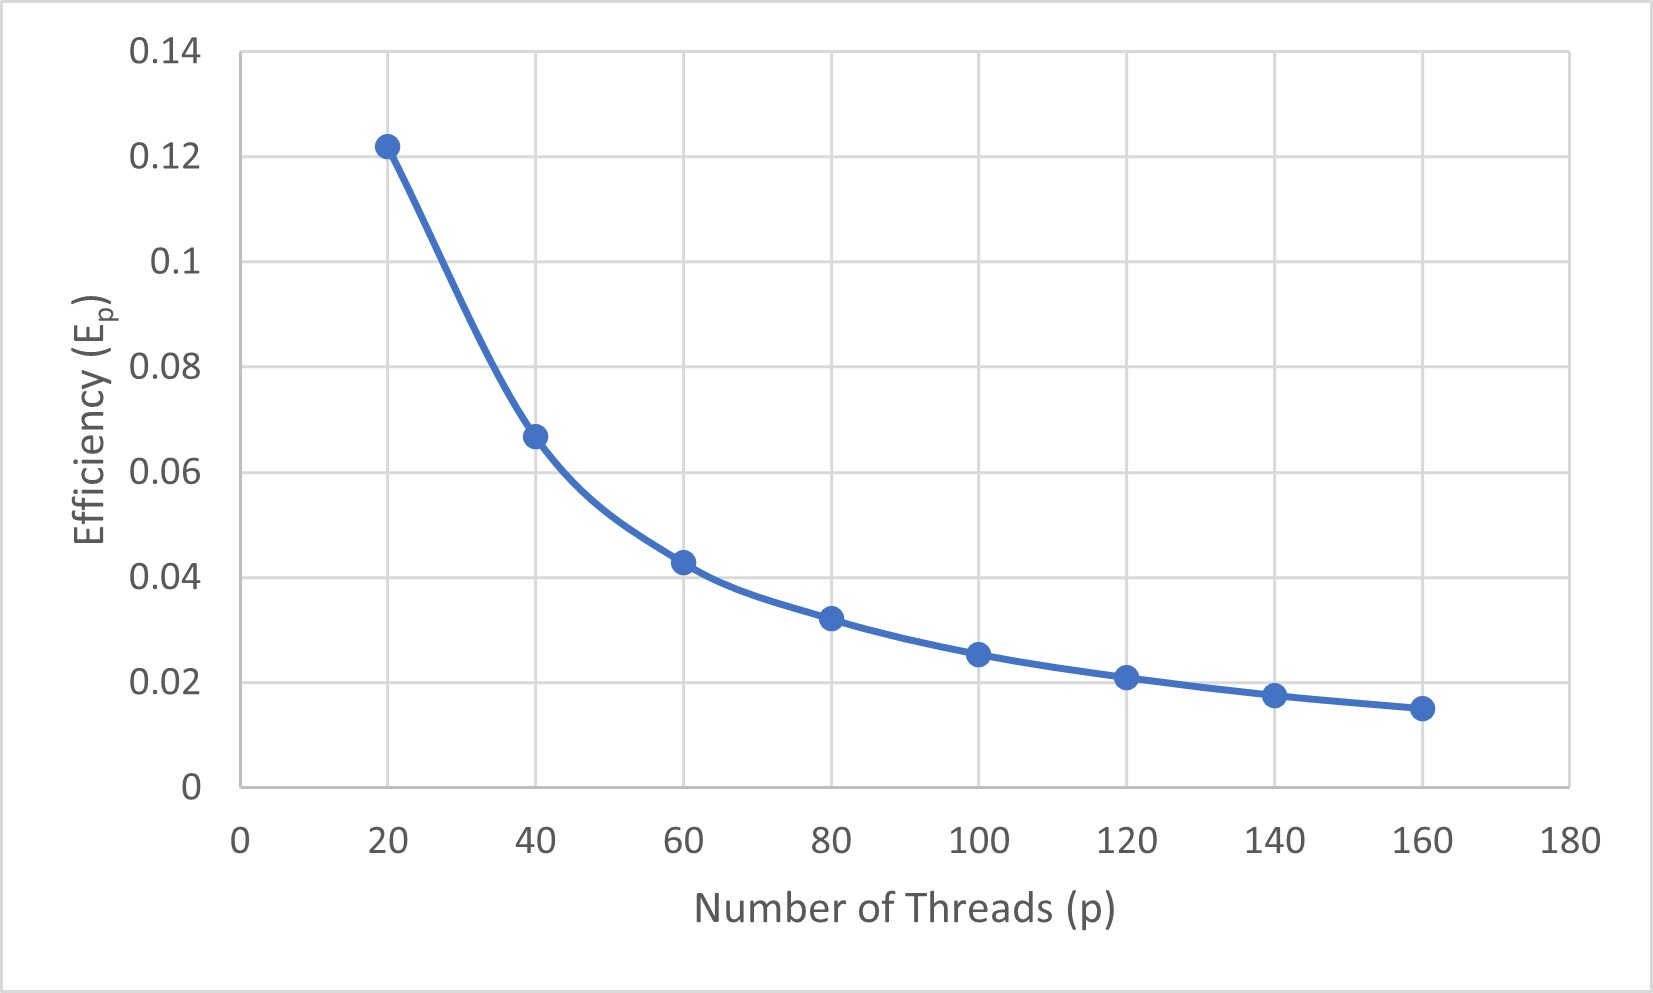
\includegraphics{Ep1}
    \caption{Graph of Efficiency using $p$ Threads for Version 1}
    \label{fig:Ep1}
\end{figure}

\begin{figure}[H]
    \centering
    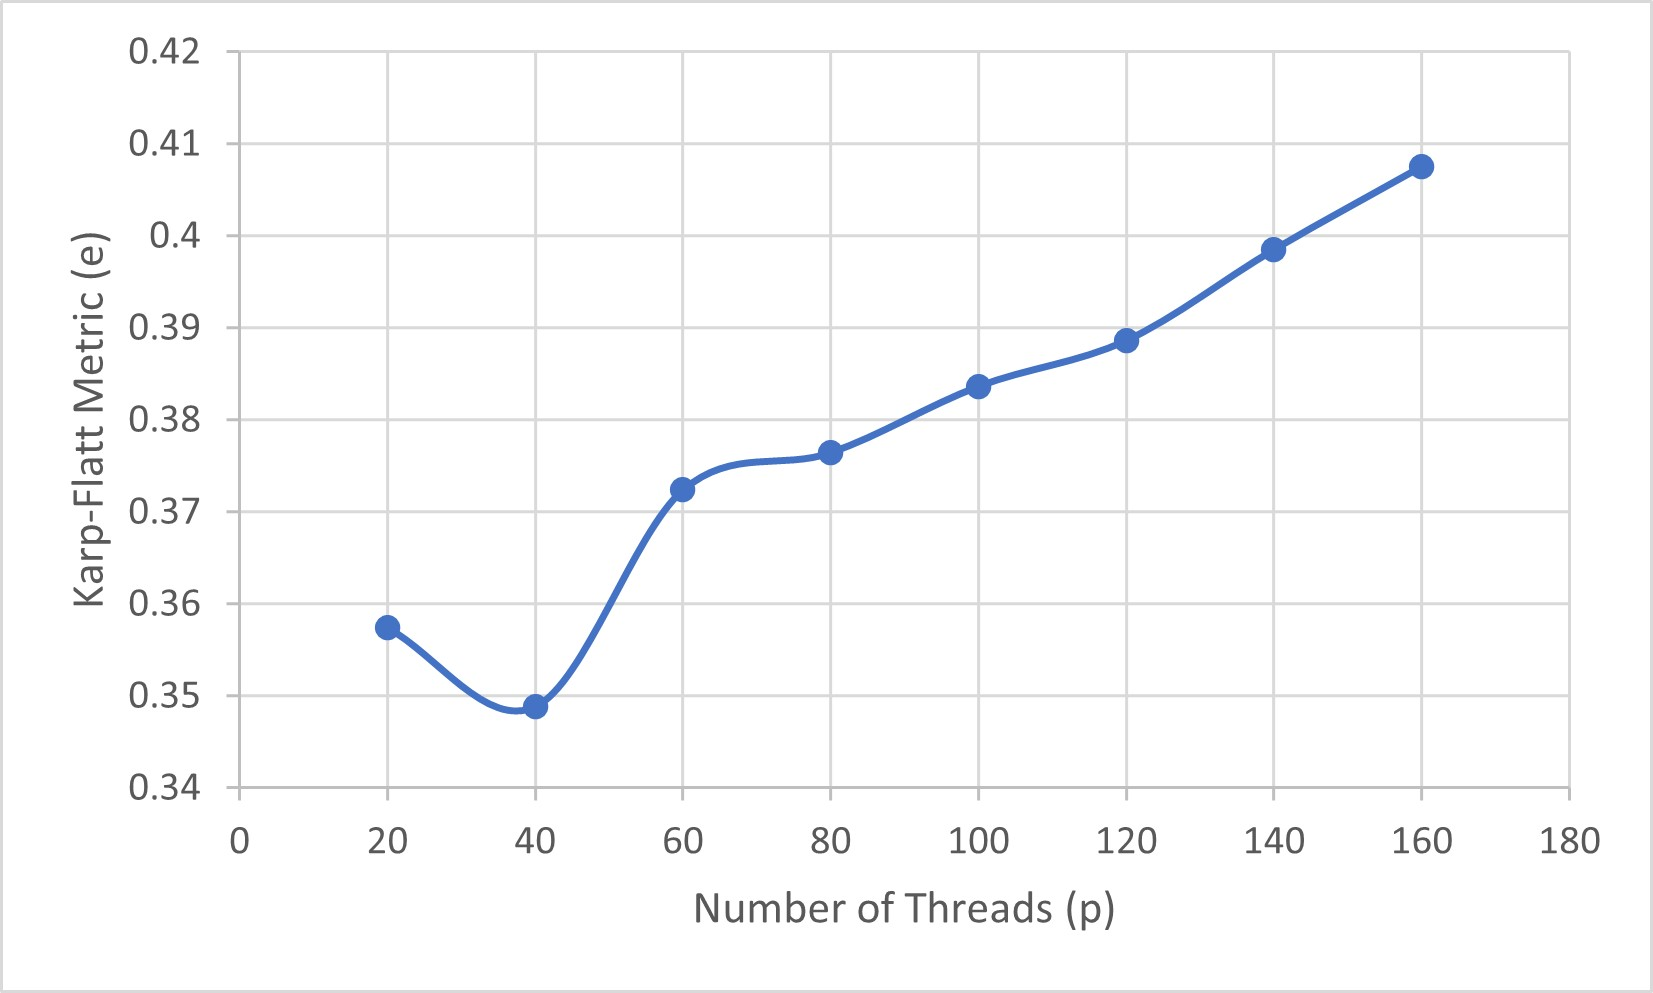
\includegraphics{kf1}
    \caption{Graph of Karp-Flatt using $p$ Threads for Version 1}
    \label{fig:kf1}
\end{figure}

\subsection{Version 2}

\subsubsection{Strategy}

It was conjectured in Section \ref{v1results} that low efficiency and Karp-Flatt was due to excessive serial computation in both the read and the write steps.

The first bottleneck was due to the serial nature of the write operation. That is, the main matrix was locked as a whole for the write of an individual element. There were two possible avenues to rectify this, detailed below.

\begin{enumerate}
    \item Use a matrix of mutual exclusions - one for each element in the matrix that can be locked and unlocked for matrix accesses.
    \item Remove the use of mutual exclusions entirely, as the batching process I have implemented inherently ensures that no unsafe accesses can occur. 
\end{enumerate}

\noindent I chose option 2, as the overhead of constantly locking and unlocking is both significant and unnecessary, for the reasons stated above.

The second bottleneck was more subtle. This arose from the serial nature of the operation that creates a copy of the main matrix for later use in the value calculation and write step. This was executing in $O(N)$ time as it was not implemented in parallel. This was addressed in Version 2, and is now parallelised using a similar batch-per-thread approach to that of the write operation.

Test runs for Version 2 were only completed using values of $p$ as multiples of 5 in the interval $(0, 40]$ to combat the efficiency dropoff observed in testing for Version 1.

\subsubsection{Analysis}

It can be observed from Tables \ref{tab:timev2} and \ref{tab:metricsv2}; and Figures \ref{fig:Sp2}, \ref{fig:Ep2}, and \ref{fig:kf2} that the changes of Version 2 effect a significant improvement in all metrics over Version 1. The general trend shown by Figure \ref{fig:Sp2} is a sharp initial speedup for $1<p\leq20$, with speedup starting to plateau for $p>20$. This is in line with what we would expect. Version 2 will serve as a suitable baseline for scalability testing in Section \ref{section:scalability}.


\begin{table}[H]
    \centering
    \begin{tabular}{cc}
    \textbf{Threads ($p$)} & \textbf{Elapsed Time ($t_p$) / s} \\ \hline
    1                      & 784.600                           \\
    5                      & 242.012                           \\
    10                     & 131.896                           \\
    15                     & 59.797                            \\
    20                     & 47.601                            \\
    25                     & 52.028                            \\
    30                     & 45.366                            \\
    35                     & 39.739                            \\
    40                     & 51.523                           
    \end{tabular}
    \caption{Mean Elapsed Time using $p$ Threads for Version 2}
    \label{tab:timev2}
\end{table}

\begin{table}[H]
    \centering
    \begin{tabular}{cccc}
    \textbf{Threads ($p$)} & \textbf{Speedup ($S_p$)} & \textbf{Efficiency ($E_p$)} & \textbf{Karp-Flatt Metric ($e$)} \\ \hline
    1 & 0.735 & 0.735 & - \\
    5 & 2.382 & 0.476 & 0.170 \\
    10 & 4.371 & 0.437 & 0.118 \\
    15 & 9.642 & 0.643 & 0.032 \\
    20 & 12.112 & 0.606 & 0.030 \\
    25 & 11.081 & 0.443 & 0.049 \\
    30 & 12.709 & 0.424 & 0.044 \\
    35 & 14.509 & 0.415 & 0.040 \\
    40 & 11.190 & 0.280 & 0.064
    \end{tabular}
    \caption{Speedup, Efficiency, and Karp-Flatt Metrics using $p$ Threads for Version 2}
    \label{tab:metricsv2}
\end{table}

\begin{figure}[H]
    \centering
    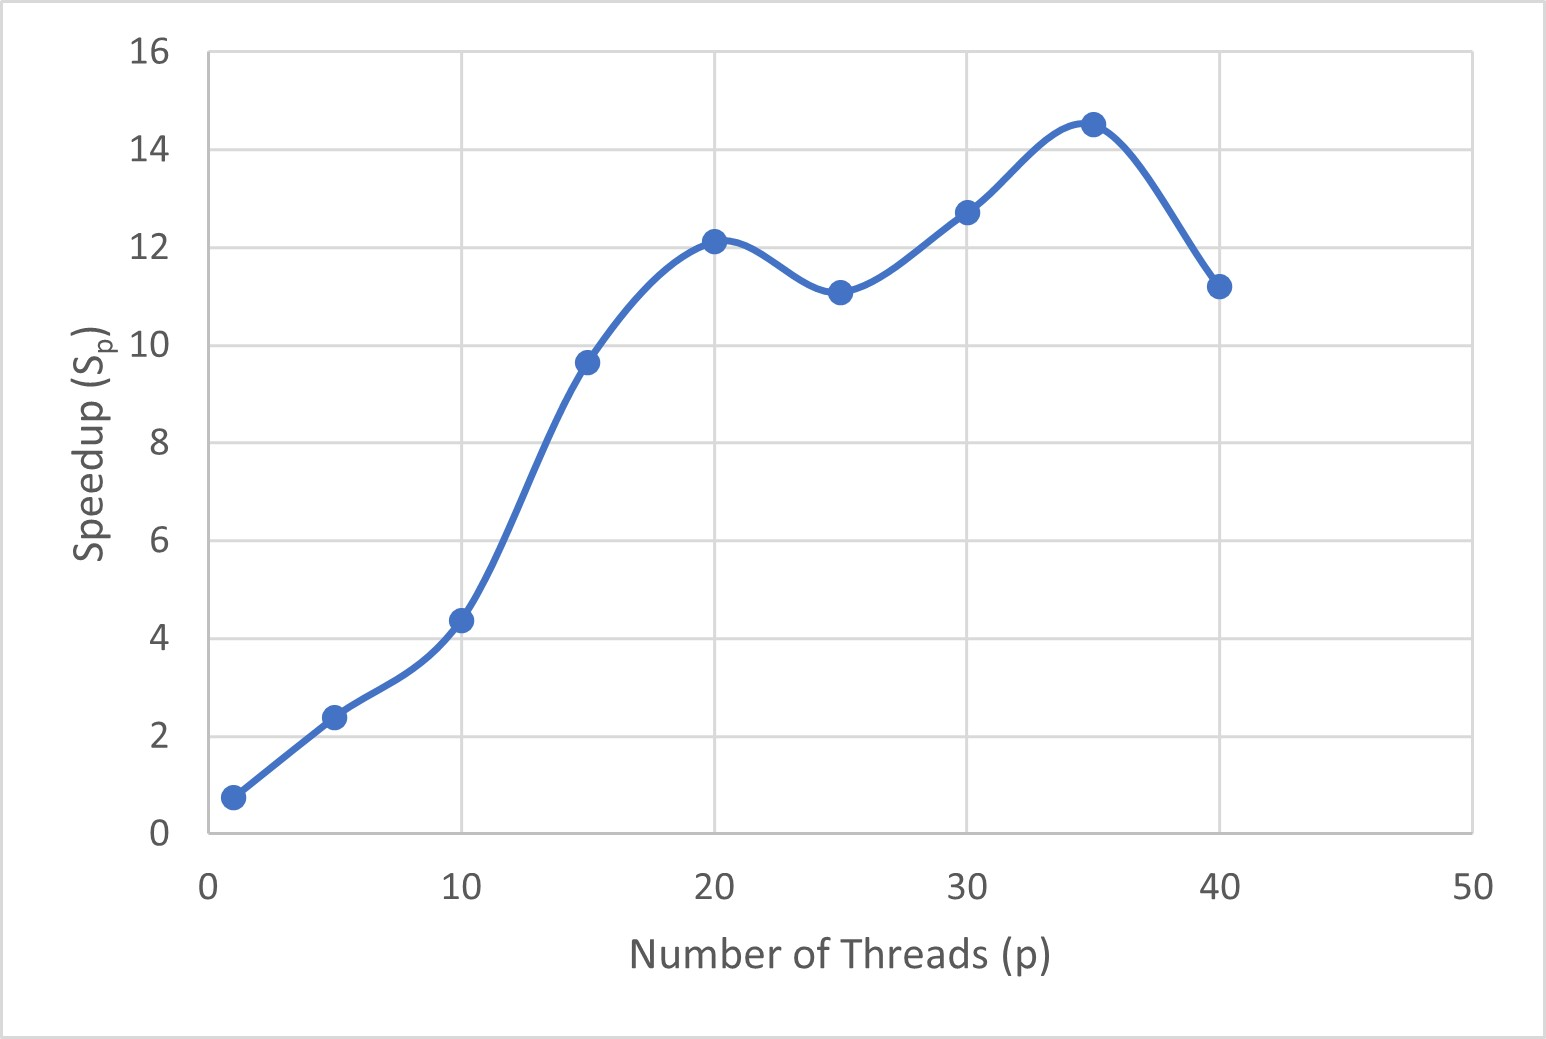
\includegraphics{Sp2}
    \caption{Graph of Speedup using $p$ Threads for Version 2}
    \label{fig:Sp2}
\end{figure}

\begin{figure}[H]
    \centering
    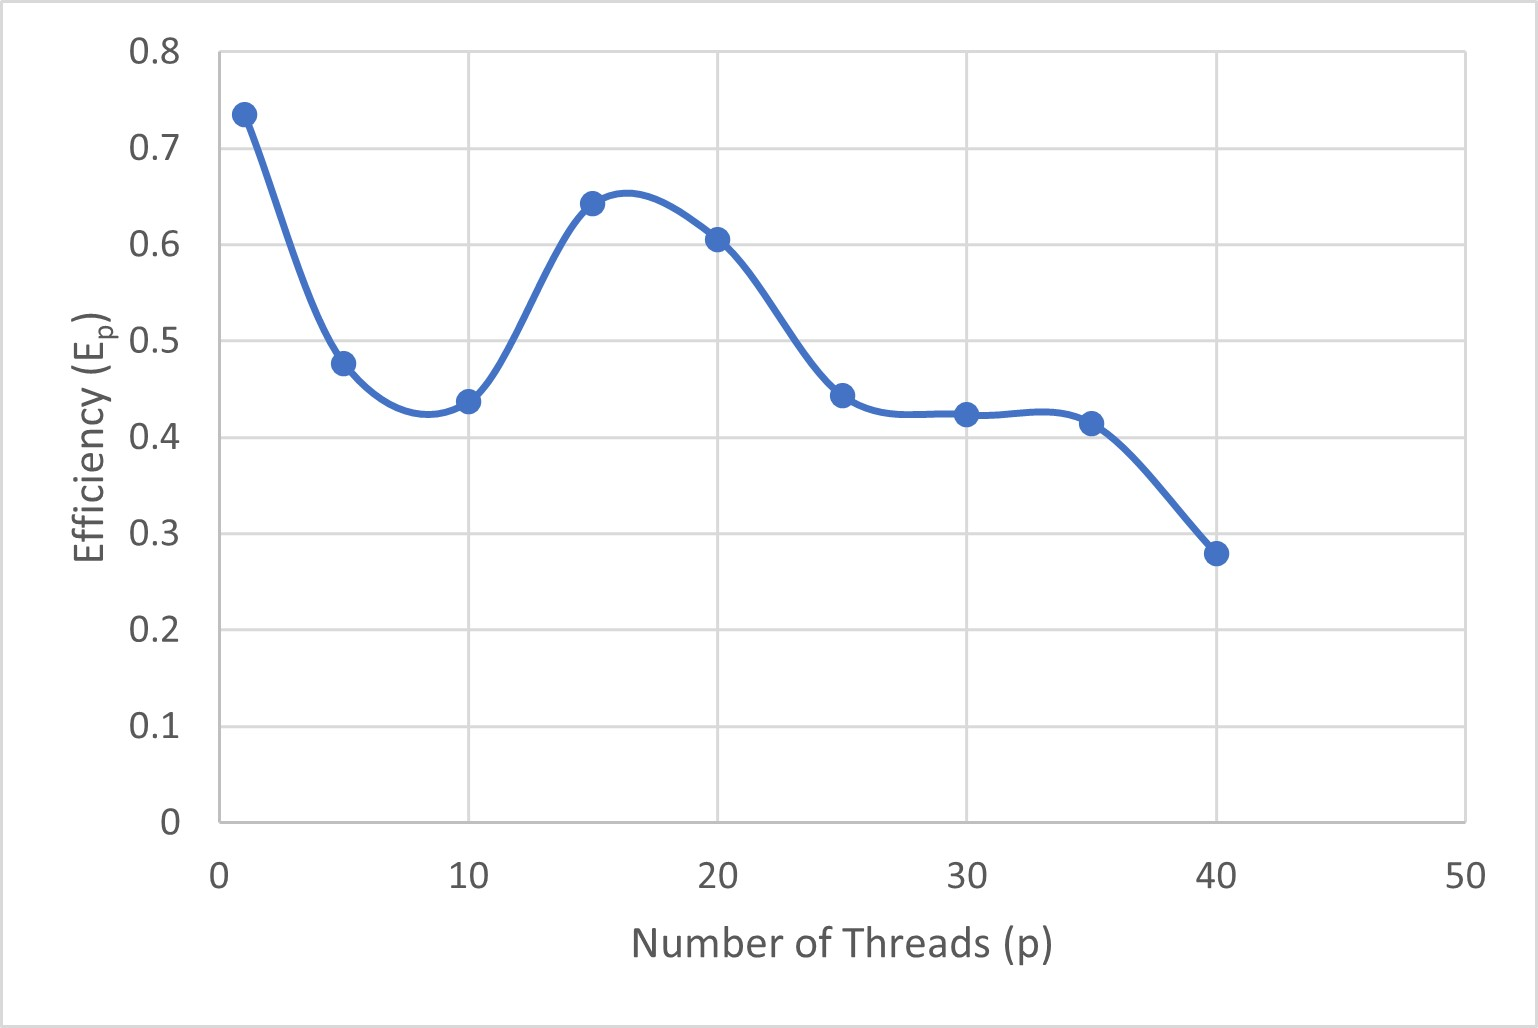
\includegraphics{Ep2}
    \caption{Graph of Efficiency using $p$ Threads for Version 2}
    \label{fig:Ep2}
\end{figure}

\begin{figure}[H]
    \centering
    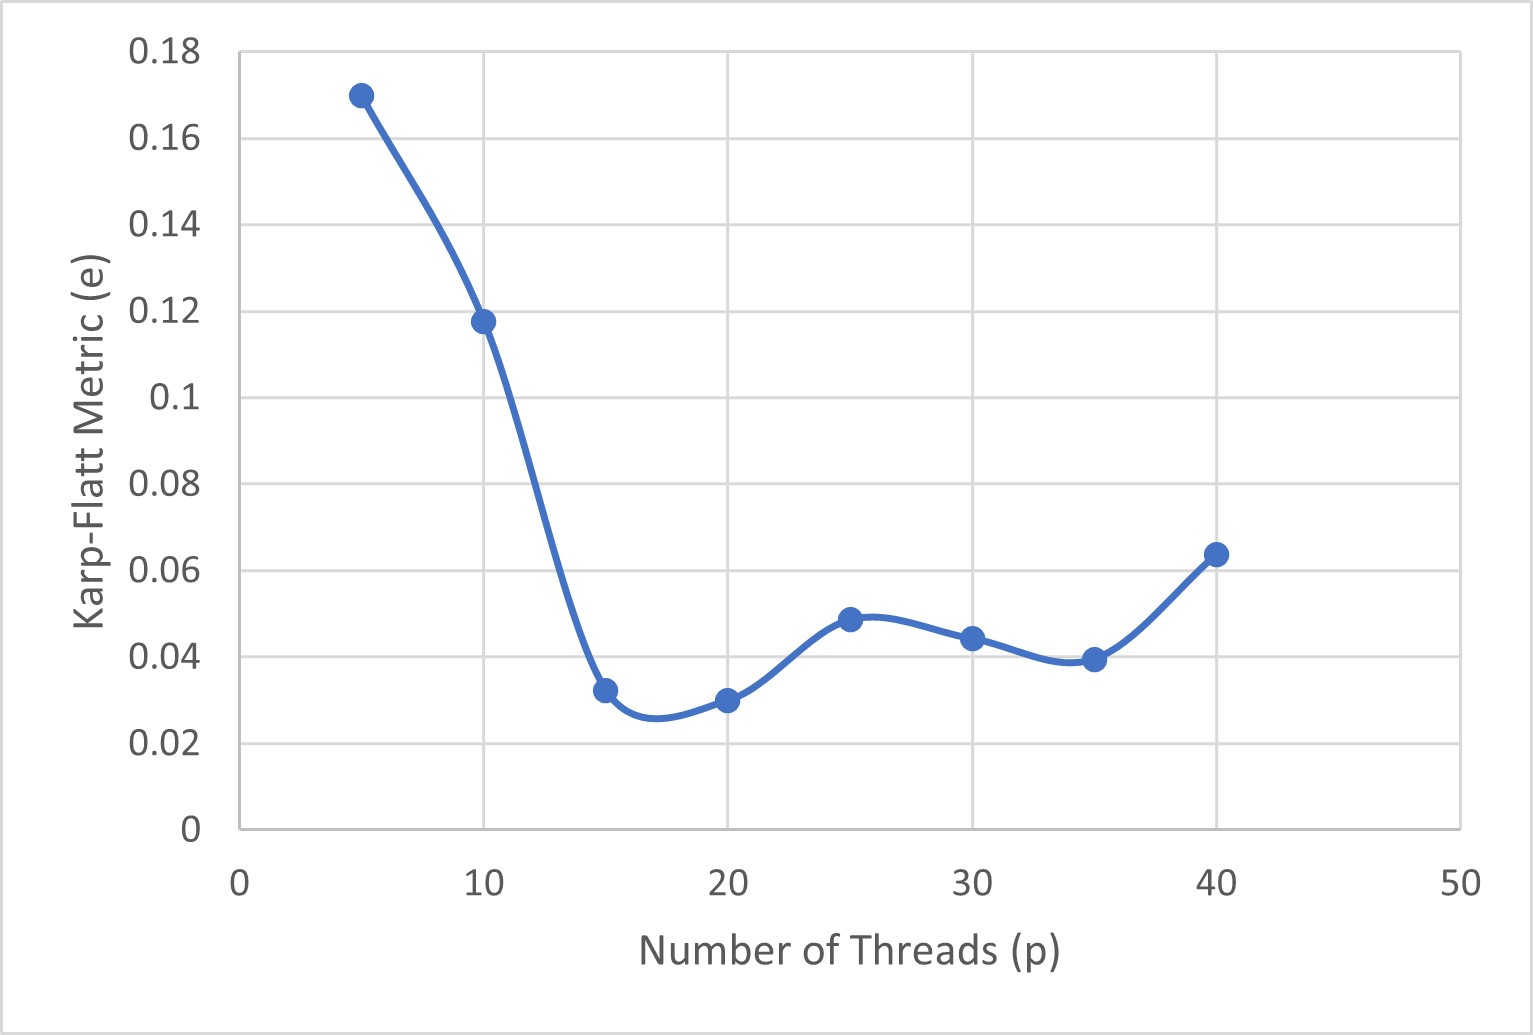
\includegraphics{kf2}
    \caption{Graph of Karp-Flatt using $p$ Threads for Version 2}
    \label{fig:kf2}
\end{figure}